\documentclass[UTF8]{article}

\usepackage{ctex}
\usepackage{marginnote}
\usepackage{listings}
\usepackage{xcolor}
\usepackage{graphicx}
\usepackage{geometry}


\title{布局}
\author{Xmp}
\date{\today}
\begin{document}
\setcounter{tocdepth}{5}
\maketitle	
\begin{abstract}
在\LaTeX 中每一个排版对象都是一个盒子。排版就是要把小盒子用空白间距粘在一起放到大盒子里,然后再依次嵌套到更大的盒子里。怎样优化这些大大小小的盒子是一门很深的学问。
\end{abstract}
\tableofcontents

\lstset
{
	numbers=left, 
	numberstyle= \tiny, 
	keywordstyle= \color{ blue!70},
	commentstyle= \color{red!50!green!50!blue!50}, 
	frame=shadowbox, % 阴影效果
	rulesepcolor= \color{ red!20!green!20!blue!20} ,
	escapeinside=``, % 英文分号中可写入中文
	xleftmargin=2em,xrightmargin=2em, aboveskip=1em,
	framexleftmargin=2em
}

\section{页面尺寸}
在排版时页面是最大的盒子。

人们在日常生活中可以见到多种规格的纸张,它们一般属于两大类标准:公制和美制。

\subsection{国际标准}
C系列的尺寸是A和B系列纸张尺寸的几何平均。

A(A0,841mm$\times$1189mm)系列常用于公文;B系列常用于海报和护照 (B7,88mm$\times$125mm);C系列常用于信封,因为它恰好比A系列大一点,比如A4纸可以装在C4信
封里,对折一下就可以装进C5信封,再对折一次装进C6信封。


\subsection{美国标准}
在1996年推出ANSIY14.1作为遮羞布。它定义了A, B, C, D, E 五种规格,A就是 Letter,B比A面积大一倍,C比B大一倍,依次类推。它们的长宽比不一致,B和C比其他三种瘦很多。它们的尺寸倒是和 A4–A0 差不多,如果不挑剔也可以混用。

\subsection{尺寸详解}
\begin{figure}[htbp]
	\centering
	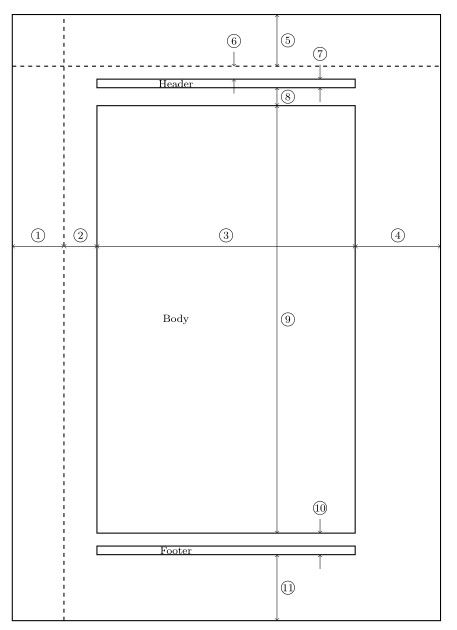
\includegraphics[width=180pt]{layout.png}
	\caption{页面尺寸}
	\label{fig:layout}
\end{figure}
\ref{fig:layout}是一张A4纸,尺寸是210mm$\times$297mm也就是597pt$\times$845pt。图中标注为Body的是正文区域,Header是页眉,Footer是页脚。

下面是会遇到的一些\LaTeX 定义的尺寸宏变量。尺寸用的是11pt,oneside的


1. 页边距,1in。在微软 Word 里这个尺寸也很常见;\\
2. \textbackslash oddsidemargin 或 \textbackslash evensidemargin,奇数或偶数页左边距,46pt;\\
3. \textbackslash textwidth,正文宽度,360pt,可以放下大概32个汉字;\\
4. 597pt减去左边的1in+46pt和中间的360pt,还剩下119pt,左右相差不到 1pt。如果双面打印的话,两面的正文部分恰好是重叠的;\\
5. 页边距,1in;\\
6. \textbackslash topmargin,上边距,18pt;\\
7. \textbackslash headheight,页眉高度,12pt;\\
8. \textbackslash headsep,页眉与正文间距,25pt;\\
9. \textbackslash textheight,正文高度,595pt,可以放下38行文字;\\
10.\textbackslash footskip,正文与页脚基线间距,30pt。它比页眉的12pt+25pt小了7pt,不理解的同学可以照照镜子,你左右是对称的,但是上下呢?\\
11. 845pt减去上面全部尺寸,还剩下93pt,比上面的1in+18pt多了3pt。\\

当字号等发生变化时,上述某些尺寸也会发生一定的变化。比如我们把oneside改成twoside,那么奇偶页的左边距就分别变成22pt和70pt。但是奇数页右边空白恰好和偶数页左边空白相等,不会给双面打印造成困扰。

一般情况下我们无须改动\LaTeX 的页面布局缺省设置。当有特殊需要时,可以使用\textbackslash setlength或\textbackslash addtolength来设置上述宏变量的值。

使用geometry宏包有更高级的用户接口。

\section{页面样式}
页面样式:页眉和页脚的内容。如下图:
\begin{figure}[htbp]
	\centering
	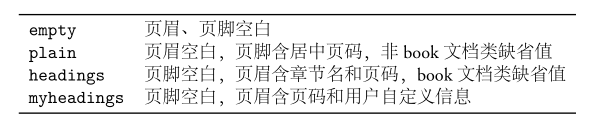
\includegraphics[width=300pt]{layout1.png}
	\caption{页面样式}
	\label{fig:layout1}
\end{figure}
\ref{fig:layou1}是通过定义四个宏变量oddhead,evenhead,oddfoot,evenfoot来设置奇偶页的页眉和页脚。

\begin{lstlisting}
\pagestyle{plain} %全局设置
\thispagestyle{empty}%单页设置
\end{lstlisting}

也可以如下代码定义。

其中第二行代码定义了permanentdamagedhead样式,定义这个特殊命令时一定要写成\textbackslash ps@style的样子;而在引用时,则写成\textbackslash pagestyle{style}。第三至六行分别定义了
奇偶页的页眉和页脚;单面文档奇偶页样式一样,所以需要且只需要定义奇数页的页眉和页脚,偶数页的定义不起作用。

这段代码中的\textbackslash hfill是个弹性填充命令,它把两边的内容“推”得尽可能远。例中使用了特殊符号@,所以要在第一行用\textbackslash makeatletter命令声明一下,暂时把它当正常符号用;用完之后,在最后一行用相应的\textbackslash makeatother命令恢复现场。

在自定义页面样式时,我们不仅可以在页眉和页脚里使用普通字符串,也可以使用一些宏变量来显示页码、章节号码和名称等.如\textbackslash thepage, thechapter, thesection, chaptername, sectionname, leftmark, rightmark。
\begin{lstlisting}
\makeatletter

\newcommand{\ps@permanentdamagedhead}{
\renewcommand{\@oddhead}{whut \hfill xmp}
\renewcommand{\@oddfoot}{\hfill\thepage\hfill}
\renewcommand{\@evenhead}{whut \hfill xmp}
\renewcommand{\@evenfoot}{\@oddfoot}
}
\makeatother	

\end{lstlisting}

关于这里的宏包有fancyhdr。

就我目前的使用情况来说,我是用内置的样式即可,不想有过深的研究。

\section{分栏}
双栏:
\begin{lstlisting}
\documentclass[twocolumn]{article}
\end{lstlisting}

使用multicol宏包有更多功能。

\section{分页}
\LaTeX 通常都会自动分页,但浮动体较多时,自动分页的效果不好。需要手工插入分页命令:
\begin{lstlisting}
\newpage
\end{lstlisting}

4表示强烈要求分页,1表示自己决定:
\begin{lstlisting}
\pagebreak[3]
\end{lstlisting}

4表示强烈反对分页,1表示自己决定:
\begin{lstlisting}
\nopagebreak[2]
\end{lstlisting}

排完此前所有浮动体:
\begin{lstlisting}
\clearpage
\end{lstlisting}


\end{document}